\documentclass[tikz]{standalone}

\usetikzlibrary{matrix,positioning,calc}

\begin{document}
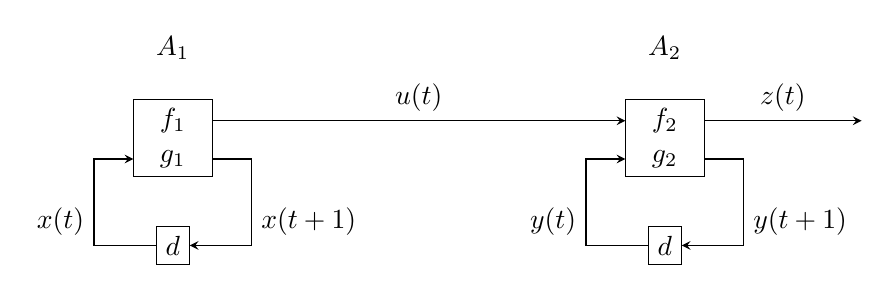
\begin{tikzpicture}[
    node distance=0cm
]
    \matrix [matrix of nodes,
            nodes={minimum width=1cm, outer sep=0cm},
            column sep=-\pgflinewidth, row sep=-\pgflinewidth] (m1) {
        \node (f1) {$f_1$}; \\
        \node (g1) {$g_1$}; \\
    };
    \node [above=0.25cm of m1] (A1) {$A_1$};
    \node [draw,below=0.5cm of m1] (d1) {$d$};

    \matrix [right=5cm of m1,
            matrix of nodes,
            nodes={minimum width=1cm, outer sep=0cm},
            column sep=-\pgflinewidth, row sep=-\pgflinewidth] (m2) {
        \node (f2) {$f_2$}; \\
        \node (g2) {$g_2$}; \\
    };
    \node [above=0.25cm of m2] (A2) {$A_2$};
    \node [draw,below=0.5cm of m2] (d2) {$d$};
    \draw (f1.north east) -- (g1.south east) -- (g1.south west) -- (f1.north west) -- cycle;
    \draw (f2.north east) -- (g2.south east) -- (g2.south west) -- (f2.north west) -- cycle;

    \draw [-stealth] (f1.east) -- node [above] {$u(t)$} (f2.west);

    \draw [-stealth] (g1.east) -- +(0.5cm, 0) |- node [above right] {$x(t+1)$} (d1.east);
    \draw [stealth-] (g1.west) -- +(-0.5cm, 0) |- node [above left] {$x(t)$} (d1.west);

    \draw [-stealth] (g2.east) -- +(0.5cm, 0) |- node [above right] {$y(t+1)$} (d2.east);
    \draw [stealth-] (g2.west) -- +(-0.5cm, 0) |- node [above left] {$y(t)$} (d2.west);

    \draw [-stealth] (f2.east) -- node [above] {$z(t)$} ($(f2.east) + (2cm, 0)$);
\end{tikzpicture}

\end{document}